%credits K. Κουνής, I. Στεφανίδου 
%refactoring : K.Draziotis (drazioti@gmail.com)
%Licence CC_BY_SA

\documentclass[12pt]{article}
\usepackage{helvet} 
\usepackage{amsmath}
\usepackage{titlesec}
\usepackage{lipsum}
\usepackage{graphicx}
\graphicspath{{images/}}


\usepackage{listings}
\usepackage{xcolor}

\definecolor{codegreen}{rgb}{0,0.6,0}
\definecolor{codegray}{rgb}{0.5,0.5,0.5}
\definecolor{codepurple}{rgb}{0.58,0,0.82}
\definecolor{backcolour}{rgb}{0.95,0.95,0.92}

\lstdefinestyle{mystyle}{
	backgroundcolor=\color{backcolour},   
	commentstyle=\color{codegreen},
	keywordstyle=\color{magenta},
	numberstyle=\tiny\color{codegray},
	stringstyle=\color{codepurple},
	basicstyle=\ttfamily\footnotesize,
	breakatwhitespace=false,         
	breaklines=true,                 
	captionpos=b,                    
	keepspaces=true,                 
	numbers=left,                    
	numbersep=5pt,                  
	showspaces=false,                
	showstringspaces=false,
	showtabs=false,                  
	tabsize=2
}
\lstset{style=mystyle}

\titleformat{\section}[display]
{\clearpage\vspace*{50pt}%
	\normalfont\huge\bfseries}%
{{\Kappa}E{\Phi}A{\Lambda}AIO \thesection}%
{20pt}%
{\Huge}%
[\vspace{40pt}]

\usepackage[algosection,commentsnumbered,ruled,vlined]{algorithm2e}
\NoCaptionOfAlgo
\usepackage{chemarrow}
\newcommand\aug{\fboxsep=-\fboxrule\!\!\!\fbox{\strut}\!\!\!}
\usepackage{graphicx}
\usepackage{gfsdidot}
\usepackage[LGR,T1]{fontenc}
\usepackage[utf8]{inputenc}
\usepackage[english,greek]{babel} % και για τις δυο γλώσσες
\usepackage{alphabeta}
\usepackage[hidelinks]{hyperref}
\usepackage{hyperref}
\usepackage{makeidx}
\usepackage{enumerate}
\usepackage{enumitem}
\usepackage{systeme}
\usepackage{algorithmic}
\usepackage{comment}

% TEXT FORMATTING
% set spacing between lines (διάστιχο)
\usepackage{setspace}
\setstretch{1.5}
% package to customize chapters, sections and subsections style
\usepackage{titlesec}
% chapter title appearance format
\titleformat{\chapter}[display]
{\bfseries\huge}{\chaptertitlename\space\thechapter}{16pt}{}
% https://www.sharelatex.com/learn/Sections_and_chapters
\titlespacing{\chapter}{0pc}{1.5ex plus .1ex minus .2ex}{5pc}
% section title appearance format
\titleformat{\section}
{\bfseries\large}{\thesection}{14pt}{}
% subsection title appearance format
\titleformat{\subsection}
{\bfseries\normalsize}{\thesubsection}{12pt}{}
% set margins
\usepackage{geometry}
\geometry{left=3cm, right=2cm, top=4cm, bottom=3cm}
\usepackage{graphicx}
% put images in images path
\graphicspath{{images/}}
\usepackage{setspace}

% Caption customization
% use this package to set appearance for captions
\usepackage{caption}
% caption size for figures 10pt
\captionsetup[figure]{font=footnotesize,labelfont=footnotesize}
% caption size for tables 10pt and underlined
\usepackage[normalem]{ulem} % Package for underlining
\DeclareCaptionLabelFormat{label_format}{\uline{#1~#2}} % underline label
\DeclareCaptionTextFormat{text_format}{\uline{#1}} % underline text
\DeclareCaptionLabelSeparator{separator_format}{\uline{:~}} % underline separator
\captionsetup[table]{font=normalsize,labelfont=normalsize,labelformat=label_format,textformat=text_format,labelseparator=separator_format}

% use this package to define custom colors
\usepackage{xcolor}

% create colors
\colorlet{punct}{red!60!black}
\definecolor{background}{HTML}{EEEEEE}
\definecolor{delim}{RGB}{20,105,176}
\colorlet{numb}{magenta!60!black}


\usepackage{amsfonts}
\usepackage{amscd}
\usepackage{amssymb}
\newtheorem{algor}{\bf{Algorithm}}[subsection]


\newtheorem{remark}{Remark}[section]

\newtheorem{theorem}{Theorem}[section]
\newtheorem{lemma}[theorem]{Lemma}
%\newtheorem{corollary}[theorem]{Corollary}
\newtheorem{definition}[theorem]{Definition}
\newtheorem{proposition}[theorem]{Proposition}
%\theoremstyle{remark}
%\newtheorem{example}[theorem]{Example}
%\newtheorem{remark}[theorem]{Remark}
\numberwithin{equation}{section}

% use this package to show actual code listings
\usepackage{listings}

% change listings name in caption to Απεικόνιση
\renewcommand{\lstlistingname}{Απεικόνιση}

% change listings name in contents page to Κατάλογος απεικονήσεων
\renewcommand\lstlistlistingname{Κατάλογος απεικονίσεων}

% set custom colorscheme for listings with language=lang1 to make them stand out more
% http://tex.stackexchange.com/questions/83085/how-to-improve-listings-display-of-json-files
\lstdefinelanguage{lang1}{
	basicstyle=\normalfont\ttfamily,
	%    numbers=left,
	%    numberstyle=\scriptsize,
	%    stepnumber=1,
	%    numbersep=8pt,
	showstringspaces=false,
	breaklines=true,
	frame=lines,
	backgroundcolor=\color{background},
	literate=
	*{0}{{{\color{numb}0}}}{1}
	{1}{{{\color{numb}1}}}{1}
	{2}{{{\color{numb}2}}}{1}
	{3}{{{\color{numb}3}}}{1}
	{4}{{{\color{numb}4}}}{1}
	{5}{{{\color{numb}5}}}{1}
	{6}{{{\color{numb}6}}}{1}
	{7}{{{\color{numb}7}}}{1}
	{8}{{{\color{numb}8}}}{1}
	{9}{{{\color{numb}9}}}{1}
	{:}{{{\color{punct}{:}}}}{1}
	{,}{{{\color{punct}{,}}}}{1}
	{\{}{{{\color{delim}{\{}}}}{1}
	{\}}{{{\color{delim}{\}}}}}{1}
	{[}{{{\color{delim}{[}}}}{1}
	{]}{{{\color{delim}{]}}}}{1},
}


% create command for blank page
\usepackage{afterpage}
\newcommand\blankpage{%
	\null
	\thispagestyle{empty}%
	\addtocounter{page}{-1}%
	\newpage}

\definecolor{maroon}{HTML}{AF3235}
% add clickable hyperlinks
\usepackage{hyperref}
\hypersetup{
	colorlinks,
	citecolor=black,
	filecolor=black,
	linkcolor=black,
	urlcolor=black
}

% use fancy header and footer
\usepackage{fancyhdr}
\usepackage{blindtext} % to quickly get a full document

% Turn on the style
\pagestyle{fancy}

% Clear the header and footer
\fancyhf{}

% Set the right side of the footer to be the page number
\fancyfoot[R]{\thepage}

% set page number appearance to bottom right
\fancypagestyle{plain}{%
	\renewcommand{\headrulewidth}{0pt}
	\fancyhf{}
	\fancyfoot[R]{\thepage}%
}

\newcommand{\HRule}{\rule{\linewidth}{0.5mm}}
\newcommand{\lt}{\latintext}

\begin{document}
	\begin{titlepage}
		
		{\LARGE Αριστοτέλειο Πανεπιστήμιο Θεσσαλονίκης}
		\begin{center} {\Large Σχολή Θετικών Επιστημών} \end{center}
		\begin{figure}[h]
			\raggedright
			\hspace{90pt}
			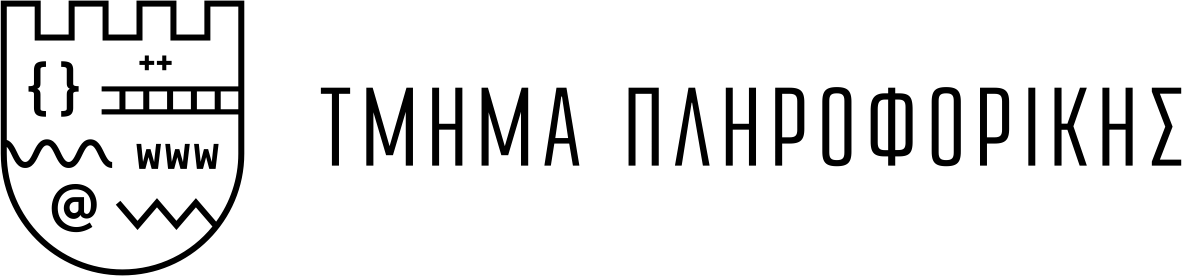
\includegraphics[width=0.5\linewidth]{logo.png}
		\end{figure}
		\begin{center}
			
			
			\begin{figure}[h]
				\centering 
				%\includegraphics[width=0.3\linewidth]{authLogo.png}
			\end{figure}
			\begin{center}
				% leave 2 cm from above text
				
				\HRule \\[0.4cm]
				{\huge Εργασία στο μάθημα της Κρυπτογραφίας}
				
				\HRule \\[0.4cm]
			\end{center}
			
			% put this on the bottom
			\vfill
			\begin{doublespacing}
				
				{\LARGE 
					Φτιάκας Σωτήριος ΑΕΜ: 3076\\}
				{\LARGE 
					Μπάρμπας Γρηγόριος ΑΕΜ: 3108\\}
				
				
				\vfill 
				{\Large \today}
			\end{doublespacing}
		\end{center}
	\end{titlepage}
	
	
	% insert table of contents
	\tableofcontents
	
	\clearpage
	
	
	\addcontentsline{toc}{section}{Περίληψη}
	\section*{{\color{maroon}Περίληψη}}
	
	..............
	% leave blank page before main part
	\blankpage
	
	\addcontentsline{toc}{section}{Θέμα 1}
	\section*{{\color{maroon}Θέμα 1}}
	\section*{\lt{RC4 \& OTP}}
	Κώδικας με σχόλια στα αρχεία:
	{\lt{
			$$No1\_i\_RC4.ipynb$$
			$$No1\_ii\_OTP.ipynb$$
	}}
	
	\addcontentsline{toc}{section}{Θέμα 2}
	\section*{{\color{maroon}Θέμα 2}}
	\section*{\lt{Avalanche Effect}}
	Κώδικας με σχόλια στο αρχείο:
	{\lt{
			$$No2\_Avalanche\_Effect.ipynb$$
	}}
	
	\addcontentsline{toc}{section}{Θέμα 3}
	\section*{{\color{maroon}Θέμα 3}}
	\section*{\lt{Vigenere}}
	Κώδικας με σχόλια στο αρχείο:
	{\lt{
		$$No3\_Vigenere.ipynb$$
	}}
	
	\addcontentsline{toc}{section}{Θέμα 4}
	\section*{{\color{maroon}Θέμα 4}}
	\section*{\lt{K,Y,E}}
	{\lt{
			Ο αριθμός κάθε γράμματος που βρίσκεται στα αριστερά προστίθεται στον αντίστοιχο αριθμό του κλειδιού, το αποτέλεσμα ανάγεται σε mod 26 και αντικαθίσταται από το γράμμα του πίνακα.\\
			Για παράδειγμα, έστω ότι το πρώτο γράμμα είναι το x. Προσθέτοντας με πιθανό κλειδί Κ = 11, έχουμε x+11. Αφού είναι 26 τα γράμματα της αγγλικής αλφαβήτας, κάνουμε x+11 mod 26. Αυτό όπως βλέπουμε μας δίνει το Α σαν κρυπτογραφημένο μήνυμα, το οποίο ισούται με 1. Επομένως x+11 mod 26 = 1. Η λύση λοιπόν για x ανάμεσα στο 1 και το 26 είναι x = 16, με 16ο γράμμα της αλφαβήτας να είναι το P. Για πιθανό κλειδί E = 5, το x = 22, άρα το γράμμα είναι το V. Για πιθανό κλειδί το Y = 25, το x = 2, άρα το γράμμα είναι το B. Παρόμοια συνεχίζουμε για κάθε κρυπτογραφημένο γράμμα.\\
			Μετά από παρατήρηση, το τελικό αποκρυπτογραφημένο μήνυμα είναι το PEACE BEGINS WITH A SMILE.
			\begin{center}
				\begin{tabular}{||c c c c||} 
					\hline
					 & K = 11 & E = 5 & Y = 25  \\ [0.5ex] 
					\hline\hline
					 A = 1 & \textbf{P}& V& B \\ 
					\hline
					 J = 10& Y&  \textbf{E}& K  \\
					\hline
					 Z = 0&O & U &  \textbf{A} \\
					\hline
					B = 2& Q& W &  \textbf{C} \\
					\hline
					P = 16& \textbf{E}& K &  Q \\  
					\hline
					 M = 13&\textbf{B} & H &  N\\  
					\hline
					D = 4& S& Y &  \textbf{E} \\  
					\hline
					 L = 12&A & \textbf{G} & M \\ 
					\hline
					H = 8& W& C &  \textbf{I}\\  
					\hline
					 Y = 25&\textbf{N} & T &  Z\\ 
					\hline
					 D = 4& \textbf{S}& Y & E \\ 
					\hline
					B = 2&Q &  \textbf{W}& C \\ 
					\hline
				 	T = 20& \textbf{I}& O & U  \\
					\hline
					S = 19 &H & N & \textbf{T}  \\
					\hline
					M = 13&B &  \textbf{H}&  N \\
					\hline
					F = 6& U& \textbf{A} &  G \\
					\hline
					D = 4& \textbf{S}& Y &  E \\
					\hline
					X = 24&\textbf{M} & S & Y  \\
					\hline
					T = 20& \textbf{I}& U &  U \\
					\hline
					Q = 17& F& \textbf{L} &  R \\
					\hline
					J = 10 & Y& \textbf{E} &  K \\
					\hline
					
				\end{tabular}
			\end{center}		
			
	}}
	
	\addcontentsline{toc}{section}{Θέμα 5}
	\section*{{\color{maroon}Θέμα 5}}
	\section*{\lt{Dictionary Attack}}
	Κώδικας με σχόλια στο αρχείο:
	{\lt{
			$$No5\_Dictionary Attack.ipynb$$
	}}
	
	\addcontentsline{toc}{section}{Θέμα 6}
	\section*{{\color{maroon}Θέμα 6}}
	\section*{\lt{LSFR}}
	Κώδικας με σχόλια στο αρχείο:
	{\lt{
			$$No6\_LSFR.ipynb$$
	}}
	
	\addcontentsline{toc}{section}{Θέμα 7}
	\section*{{\color{maroon}Θέμα 7}}
	\section*{\lt{Shift Operator with XOR}}
	{\lt{
			m: 16-bits
			$$c=m\oplus(m<<6)\oplus(m<<10)$$
				
			Όπου $m<<a$ είναι κύλιση προς τα αριστερά κατά $a$-bits.
			
			Για μήνυμα $m$ και κλειδί $k$ ισχύει:
			Αν $c = m \oplus k$, τότε $m = c \oplus k$ 
				
			Επιπλέον, στην αρχική μας συνάρτηση κρυπτογράφησης, μπορούμε να κυλίσουμε και τα δύο μέλη ταυτόχρονα.
			$$(c<<2) = (m\oplus(m<<6)\oplus(m<<10))<<2$$
			
			$$\Leftrightarrow (c<<2) = (m<<2)\oplus(m<<8)\oplus(m<<12)$$
				
			Σημείωση: το $x<<i$ θα συμβολίζεται ως $x_i$ για ευκολία. \newline
			Συνεπώς θα έχουμε:	
			\begin{gather*} 
			c_0 = m_0 \oplus m_6 \oplus m_{10} \quad (1) \\
			c_2 = m_2 \oplus m_8 \oplus m_{12} \Rightarrow m_8 = m_2 \oplus m_{12} \oplus c_2 \quad (4) \\
			c_4 = m_4 \oplus m_{10} \oplus m_{14} \Rightarrow m_{10} = m_4 \oplus m_{14} \oplus c_4 \quad (2) \\
			c_6 = m_6 \oplus m_{12} \oplus m_0 \quad (5) \\
			c_8 = m_8 \oplus m_{14} \oplus m_2 \\
			c_{10} = m_{10} \oplus m_0 \oplus m_4 \\
			c_{12} = m_{12} \oplus m_2 \oplus m_6 \\
			c_{14} = m_{14} \oplus m_4 \oplus m_8 \Rightarrow m_{14} \oplus m_4 = m_8 \oplus c_{14} \quad (3) \\
			\end{gather*}
			
			Ξεκινώντας από την (1) έχουμε διαδοχικά:
			\begin{gather*} 
			c_0 = m_0 \oplus m_6 \oplus m_{10} \\ 
			(2)\Rightarrow c_0 = m_0 \oplus m_6 \oplus m_4 \oplus m_{14} \oplus c_4 \\
			(3)\Rightarrow c_0 \oplus c_4 = m_0 \oplus m_6 \oplus m_8 \oplus c_{14} \\
			(4)\Rightarrow c_0 \oplus c_4 \oplus c_{14} = m_0 \oplus m_6 \oplus m_2 \oplus m_{12} \oplus c_2 \\
			(5)\Rightarrow c_0 \oplus c_4 \oplus c_{14} \oplus c_2 = m_2 \oplus c_6 \\
			\Rightarrow c_0 \oplus c_4 \oplus c_{14} \oplus c_2 \oplus c_6 = m_2 \quad (6)
			\end{gather*}
			
			Κάνουμε κύλιση και στα δύο μέρη του (6) προς τα δεξιά και έχουμε:
			$$m_0 = c_{14} \oplus c_2 \oplus c_{12} \oplus c_0 \oplus c_4$$
			
			και άρα τελικά έχουμε: $$m_0 = c_0 \oplus c_2 \oplus c_4 \oplus c_{12} \oplus c_{14}$$
	}}
	Κώδικας με σχόλια στο αρχείο:
	{\lt{
			$$No7\_Shift\_Operator.ipynb$$
	}}
	
	\addcontentsline{toc}{section}{Θέμα 8}
	\section*{{\color{maroon}Θέμα 8}}
	\section*{\lt{GCD Greatest Common Divisor}}
	{\lt{
			\begin{enumerate}[label=(\roman*)]
				\item Διαιρώ το 126048 με το 5050 και έχω 126048 = 5050 $\cdot$ 24 + 4848. Κατόπιν διαιρώ τον διαιρέτη, δηλαδή το 5050 με το υπόλοιπο, δηλαδή με το 4848 και έχουμε 5050 = 4848 $\cdot$ 1 + 202. Τέλος, συνεχίζοντας όπως προηγουμένως έχω 4848 = 24 $\cdot$ 202 + 0. Το τελευταίο μη μηδενικό υπόλοιπο, δηλαδή το 202 είναι ο ΜΚΔ των αριθμών.
				
				Για τους αριθμούς Bezout έχουμε: \\
				202 = 5050 - 4848 = 5050 - (126048 - 24 $\cdot$ 5050) = \textbf{-1} $\cdot$ 126048 + \textbf{25} $\cdot$ 5050 \\
				Άρα, οι αριθμοί Bezout είναι οι: \textbf{-1}, \textbf{25}\\
				$Z_{1001} , x=809$
				\item \begin{gather*} 
				1001 = 809 \cdot 1 + 192\\
				809 = 192 \cdot 4 + 41\\
				192 = 41 \cdot 4 + 28\\
				41 = 28 \cdot 1 + 13\\
				28 = 13 \cdot 2 + 2\\
				13 = 2 \cdot 6 + 1\\
				\end{gather*}
				\begin{gather*}
				1 = 13 - 2 \cdot 6 = \\
				13 - (28 - 13 \cdot 2) \cdot 6 =\\
				13 \cdot 13 - 28 \cdot 6 =\\
				13 \cdot (41 - 281) - 28 \cdot 6=\\
				13 \cdot 41 - 28 \cdot 13 - 28 \cdot 6=\\
				13 \cdot 41 + 28 \cdot  (-19)=\\
				13 \cdot 41 + (192 - 41 \cdot 4) \cdot (-19)=\\
				13 \cdot 41 + 192 \cdot (-19) + 41 \cdot 76=\\
				\end{gather*}
				\begin{gather*}
				89 \cdot 41 + 192 \cdot (-19) =\\
				89 \cdot (809 - 192 \cdot 4) + 192 \cdot (-19)=\\
				89 \cdot 809 - 192 \cdot 356 + 192 \cdot (-19)=\\
				89 \cdot 809 + 192 \cdot (-375)=\\
				89 \cdot 809 + (1001 - 809 \cdot 1) \cdot (-375) =\\
				89 \cdot 809 + 1001 \cdot (-375) + 809 \cdot (375)=\\
				464 \cdot 809 + 1001 \cdot (-375)\\\\
				1 \equiv 464 \cdot 809 \mod 1001\\
				\end{gather*}
				
				Άρα το αντίστροφο του 809 στο $Ζ_{1001}$ είναι το 464.
				
				\item Ξέρουμε από το μικρό θεώρημα του Fermat ότι:
				$$n^{p-1} \equiv 1 \mod p$$
				δηλαδή $2^{100} \equiv 1 \mod 101$ \\
				άρα $2^{100} \equiv 1$
			\end{enumerate}			
	}}

	\addcontentsline{toc}{section}{Θέμα 9}
	\section*{{\color{maroon}Θέμα 9}}
	\section*{\lt{Entropy}}
	{\lt{
		Αρχικά υπολογίζουμε
		\begin{gather*} 
			p_x(X=0) = \sum_{y}p_{X,Y}(0,y)=\frac{3}{7} \\
			p_x(X=1) = \sum_{y}p_{X,Y}(1,y)=\frac{2}{7} \\
			p_x(X=2) = \sum_{y}p_{X,Y}(2,y)=\frac{2}{7} \\
			p_y(Y=0) = \sum_{y}p_{X,Y}(x,0)=\frac{3}{7} \\
			p_y(Y=1) = \sum_{y}p_{X,Y}(x,1)=\frac{2}{7} \\
			p_y(Y=2) = \sum_{y}p_{X,Y}(x,2)=\frac{2}{7}
		\end{gather*}
		
		Ισχύει ότι:
		$$H(X) = -\sum_{x}p_{X}(x)\log _{2}p_{X}(x) $$
		
		Επομένως
		\begin{gather*} 
			H(X) = -\frac{3}{7}\log _{2}\frac{3}{7} - \frac{2}{7}\log _{2}\frac{2}{7} - \frac{2}{7}\log _{2}\frac{2}{7} \\
			= -\frac{3}{7}\log _{2}\frac{3}{7} -\frac{4}{7}\log _{2}\frac{2}{7} \\
			\simeq 1.5566567074628228\\
			\\		
			Υ(Χ) = -\frac{3}{7}\log _{2}\frac{3}{7} - \frac{2}{7}\log _{2}\frac{2}{7} - \frac{2}{7}\log _{2}\frac{2}{7} \\
			= -\frac{3}{7}\log _{2}\frac{3}{7} -\frac{4}{7}\log _{2}\frac{2}{7} \\
			\simeq 1.5566567074628228
		\end{gather*}
		
		Επίσης έχουμε τον εξής τύπο
		$$H(X,Y)=-\sum_{x}\sum_{y}p(x,y)\log_{2}p(x,y)$$
		Άρα θα έχουμε:
		\begin{gather*} 
			Η(X,Υ) = - p(0,0)\log_{2}p(0,0) - p(0,1)\log_{2}p(0,1) - p(0,2)\log_{2}p(0,2) - \\ p(1,0)\log_{2}p(1,0) - p(1,1)\log_{2}p(1,1) - p(1,2)\log_{2}p(1,2) - \\
			p(2,0)\log_{2}p(2,0) -  p(2,1)\log_{2}p(2,1) - p(2,2)\log_{2}p(2,2) \\
			\simeq 2.5216406363433186
		\end{gather*}
		
		Θα υπολογίσουμε την $H(Y|X)$.
		Χρειαζόμαστε αρχικά τα παρακάτω,
		\begin{gather*} 
			p_{Y|X}(y=0|x=0) = \frac{p_{X,Y}(0,0)}{p_{X}(0)} = \frac{\frac{1}{7}}{\frac{3}{7}} =\frac{1}{3} \\
			p_{Y|X}(y=1|x=0) = \frac{p_{X,Y}(0,1)}{p_{X}(0)} = \frac{0}{\frac{3}{7}} = 0 \\
			p_{Y|X}(y=2|x=0) = \frac{p_{X,Y}(0,2)}{p_{X}(0)} = \frac{\frac{2}{7}}{\frac{3}{7}} =\frac{2}{3} \\
			p_{Y|X}(y=0|x=1) = \frac{p_{X,Y}(1,0)}{p_{X}(1)} = \frac{\frac{1}{7}}{\frac{2}{7}} =\frac{1}{2} \\
			p_{Y|X}(y=1|x=1) = \frac{p_{X,Y}(1,1)}{p_{X}(1)} = \frac{\frac{1}{7}}{\frac{2}{7}} =\frac{1}{2} \\
			p_{Y|X}(y=2|x=1) = \frac{p_{X,Y}(1,2)}{p_{X}(1)} = \frac{0}{\frac{2}{7}} = 0 \\
			p_{Y|X}(y=0|x=2) = \frac{p_{X,Y}(2,0)}{p_{X}(2)} = \frac{\frac{1}{7}}{\frac{2}{7}} =\frac{1}{2} \\
			p_{Y|X}(y=1|x=2) = \frac{p_{X,Y}(2,1)}{p_{X}(2)} = \frac{\frac{1}{7}}{\frac{2}{7}} =\frac{1}{2} \\
			p_{Y|X}(y=2|x=2) = \frac{p_{X,Y}(2,2)}{p_{X}(2)} = \frac{0}{\frac{2}{7}} = 0
		\end{gather*}		
	}}

	Τώρα πρέπει να υπολογίσουμε τα παρακάτω: 
	\begin{gather*} 
		H(Y|X=0) = - \sum_{y}p_{Y|X}(y|x=0)\log_{2}p_{Y|X}(y|x=0) \\
		= -(\frac{1}{3}\log_{2}\frac{1}{3} + 0 + \frac{2}{3}\log_{2}\frac{2}{3}) \\
		= -(\frac{1}{3}\log_{2}\frac{1}{3} + \frac{2}{3}\log_{2}\frac{2}{3}) \\
		H(Y|X=1) = - \sum_{y}p_{Y|X}(y|x=1)\log_{2}p_{Y|X}(y|x=1) \\
		= -(\frac{1}{2}\log_{2}\frac{1}{2} + \frac{1}{2}\log_{2}\frac{1}{2} + 0) \\
		= - \log_{2}2 = 1\\
		H(Y|X=2) = - \sum_{y}p_{Y|X}(y|x=2)\log_{2}p_{Y|X}(y|x=2) \\
		= - \log_{2}2 = 1\\
	\end{gather*}
	
	Τότε θα έχουμε
	\begin{gather*} 
		H(Y|X) = \sum_{x}p_{X}xH(Y|X=x) \\
		= p_{X}(0)H(Y|X=0) + p_{X}(1)H(Y|X=1) + p_{x}(2)H(Y|X=2) \\
		\simeq 0.9649839288804954
	\end{gather*}
	
	Γνωρίζουμε επίσης ότι από το θεώρημα της αμοιβαίας πληροφορίας έχουμε
	$$I(X,Y) = H(X) - H(X|Y) = H(Y) - H(Y|X)$$
	
	Άρα έχουμε
	\begin{gather*} 
		H(X|Y) = -(H(Y) - H(Y|X) - H(X)) \\
		\simeq 0.9649839288804954 
	\end{gather*}
	
	Τέλος,
	\begin{gather*} 
		ρ = 1 - \frac{H(Y|X)}{H(X)} \\
		\simeq 0.5916727785823274
	\end{gather*}
	
	Κώδικας με σχόλια στο αρχείο:
	{\lt{
			$$No9\_Entropy.ipynb$$
	}}
	
	\addcontentsline{toc}{section}{Θέμα 10}
	\section*{{\color{maroon}Θέμα 10}}
	\section*{\lt{Textbook RSA}}
	Κώδικας με σχόλια στο αρχείο:
	{\lt{
			$$No10\_Textbook\_RSA.ipynb$$
	}}
	
	\addcontentsline{toc}{section}{Θέμα 11}
	\section*{{\color{maroon}Θέμα 11}}
	\section*{\lt{Wiener RSA}}
	Κώδικας με σχόλια στο αρχείο:
	{\lt{
			$$No11\_Wiener\_RSA.ipynb$$
	}}
	
	\addcontentsline{toc}{section}{Θέμα 12}
	\section*{{\color{maroon}Θέμα 12}}
	\section*{\lt{Prime Numbers}}
	Κώδικας με σχόλια στο αρχείο:
	{\lt{
			$$No12\_Prime\_Numbers.ipynb$$
	}}
	
	\addcontentsline{toc}{section}{Θέμα 13}
	\section*{{\color{maroon}Θέμα 13}}
	\section*{\lt{Chinese Theorem}}
	{\lt{
			Έχουμε το σύστημα των γραμμικών ισοδυναμιών
			\begin{gather*} 
				x \equiv 9 \pmod{19} \\
				x \equiv 9 \pmod{12} \\
				x \equiv 13 \pmod{19}
			\end{gather*}
			
			Έχουμε ότι ισχύει $\gcd(12,17,19) = 1$, άρα δεν απαιτείται κάποια απλοποίηση.
			
			Για την επίλυση του συστήματος χρησιμοποιούμε το Κινέζικο Θεώρημα Υπολοίπων
			
			Έτσι έχουμε: $m=17*12*19=3876$
			
			\begin{gather*} 
				M_1 = 228y_1 \equiv 1 \mod{17} \implies 7y_1 \equiv \mod{17} \implies y_1=5 \\
				M_2 = 323y_2 \equiv 1 \mod{12} \implies 11y_1 \equiv \mod{12} \implies y_1=11 \\
				M_3 = 204y_3 \equiv 1 \mod{19} \implies 14y_1 \equiv \mod{19} \implies y_1=15
			\end{gather*}
			
			Τώρα πολλαπλασιάζουμε και προσθέτουμε:
			\begin{gather*}
				x = 9*228*5 + 9*323*11 + 13*204*15 \\
				= 82017 (1)
			\end{gather*}
			Παρατηρούμε ότι η (1) γράφεται,
			$$x = 82017 = 621 + 3876k, k \in \mathbb{Z} $$
			
			Για $k=0$ έχουμε λύση το $x=621$
	}}

	Κώδικας με σχόλια στο αρχείο:
	{\lt{
			$$No13\_ChineseTheorem.ipynb$$
	}}
	
	\addcontentsline{toc}{section}{Θέμα 14}
	\section*{{\color{maroon}Θέμα 14}}
	\section*{\lt{Miller-Rabin Test}}
	{\lt{
			\begin{enumerate}
				\item We can see that a big portion of the total numbers generated from $f(x) = x^2 + x - 1354363$, about 2/5 of the total, are primes
				\item A lucky number of Euler is a number p such that the prime-generating polynomial:\\
				        $n^2 - n + p$ is prime for $n=1, 2, ..., p-1$
				
				Specifically, the lucky numbers of Euler (excluding the trivial case $p=3$) are those numbers p such that the 
				imaginary quadratic field Q(sqrt(1-4p)) has class number 1.
				(Rabinowitz 1913, Le Lionnais 1983, Conway and Guy 1996, Ribenboim 2000).
				
				As proved by Heegner (1952) (although his proof was not accepted as complete at the time) and subsequently established by 
				Stark (1967), there are only nine numbers -d such that h(-d)=1 (the Heegner numbers -2, -3, -7, -11, -19, -43, -67, and -163), 
				and of these, only 7, 11, 19, 43, 67, and 163 are of the required form.
				
				Therefore, the only lucky numbers of Euler are 2, 3, 5, 11, 17, and 41 (Le Lionnais 1983, OEIS A014556), and
				\textbf{there does not exist a better prime-generating polynomial of Euler's form}.
			\end{enumerate}
	}}
	Κώδικας με σχόλια στο αρχείο:
	{\lt{
			$$No12\_Miller-Rabin\_Test.ipynb$$
	}}
	
	\addcontentsline{toc}{section}{Θέμα 15}
	\section*{{\color{maroon}Θέμα 15}}
		\section*{\lt{Rabin TDF}}
	Κώδικας με σχόλια στο αρχείο:
	{\lt{
			$$No15\_Rabin\_TDF.ipynb$$
	}}
	
	\addcontentsline{toc}{section}{Θέμα 16}
	\section*{{\color{maroon}Θέμα 16}}
	\section*{\lt{GPG, PGP, Send Message}}
	{\lt{
		Μπάρμπας Γρηγόριος: $$b641ed06419f8ff4a6447cc9fb9d2295$$
		
		Φτιάκας Σωτήριος: $$5f816b4f295dc95721a7a34b9fd1653a$$
	}}
	
	\addcontentsline{toc}{section}{Θέμα 17}
	\section*{{\color{maroon}Θέμα 17}}
		\section*{\lt{TDF: CRT-RSA}}
	Κώδικας με σχόλια στο αρχείο:
	{\lt{
			$$No17\_TDF\_CRT-RSA.ipynb$$
	}}

	\addcontentsline{toc}{section}{Θέμα 18}
	\section*{{\color{maroon}Θέμα 18}}
	\section*{\lt{secure.zip}}
	{\lt{
			$$9e94b15ed312fa42232fd87a55db0d39$$
	}}
	
	\addcontentsline{toc}{section}{Θέμα 19}
	\section*{{\color{maroon}Θέμα 19}}
		\section*{\lt{OpenSSL}}
	Κώδικας με σχόλια στο αρχείο:
	{\lt{
			$$No19\_OpenSSL.ipynb$$
	}}
	
	\addcontentsline{toc}{section}{Θέμα 20}
	\section*{{\color{maroon}Θέμα 20}}
		\section*{\lt{/dev/random}}
	Κώδικας με σχόλια στο αρχείο:
	{\lt{
			$$No12\_dev\_random\_entropy.ipynb$$
	}}
	
	\addcontentsline{toc}{section}{Θέμα 21}
	\section*{{\color{maroon}Θέμα 21}}
		\section*{\lt{Bibliography}}
	\begin{enumerate}
		\item \textbf{Nα αναλύσετε πως η χρήση του ίδιου κλειδιού στον {\lt{OTP}} επιτρέπει να βρούμε μηνύματα που είναι γραμμένα σε κάποια φυσική γλώσσα.}\\
		Το {\lt{OTP}} αποτελεί ένα {\lt{stream cipher}} ο οποίος αποτελεί μια {\lt{perfectly secure}} μέθοδο κρυπτογράφησης. Είναι πολύ εύκολος στην υλοποίησή του και είναι {\lt{perfectly secure}} εάν το μήκος του κλειδιού που χρησιμοποιείται είναι μεγαλύτερο ή ίσο του μήκους του μηνύματος που κρυπτογραφείται. Ωστόσο, απαιτεί επίσης το κλειδί να μην χρησιμοποιηθεί πάνω από μία φορά. Ας δούμε ένα παράδειγμα του πως μπορούμε να εξάγουμε πληροφορία από δύο κρυπτογραφημένα μηνύματα που έχουν κρυπτογραφηθεί χρησιμοποιώντας το ίδιο κλειδί.
		Έστω ότι έχουμε τα εξής:
		\begin{itemize}
			\item {\lt{message1 = "Hello World"}}
			\item {\lt{message2 = "the program"}}
			\item {\lt{key = "supersecret"}}
		\end{itemize}
		Αν μετατρέψουμε κάθε μήνυμα σε hex strings, και τα κρυπτογραφήσουμε χρησιμοποιώντας το ίδιο κλειδί, θα πάρουμε τα εξής {\lt{cipher-texts}}:
		\begin{itemize}
			\item {\lt{cipher-text1: "3b101c091d53320c000910"}}
			\item {\lt{cipher-text2: "071d154502010a04000419"}}
		\end{itemize}
		
		Ακολουθούμε λοιπόν την εξής διαδικασία:
		\begin{enumerate}
			\item Μαντεύουμε μια λέξη που μπορεί να υπάρχει σε κάποιο από τα αρχικά μηνύματα.
			\item Μετατρέπουμε τη λέξη σε {\lt{hex string}}.
			\item Κάνουμε {\lt{XOR}} τα δύο {\lt{cipher-texts}}.
			\item Κάνουμε {\lt{XOR}} το {\lt{hex string}} που δημιουργήσαμε στο βήμα 2 με το {\lt{hex string}} που δημιουργήσαμε στο βήμα 3.
			\item Αν το αποτέλεσμα είναι λέξη φυσικής γλώσσας, τότε έχουμε καταφέρει να αποσπάσουμε πληροφορία και για τα δύο αρχικά μηνύματα.
			\item  Αν δεν είναι λέξη φυσικής γλώσσας, τότε συνεχίζουμε να κάνουμε {\lt{XOR}}, μετακινόντας τη λέξη μας κάθε φορά ένα βήμα δεξιά.
		\end{enumerate}
	
		\textbf{Το βήμα 1} φαίνεται δύσκολο, δηλαδή το να μαντέψουμε κάποια λέξη σε κάποιο από τα δύο κείμενα, αλλά αν σκεφτούμε έξυπνα, μπορούμε να βελτιώσουμε τις πιθανοτητές μας. Για παράδειγμα, η λέξη {\lt{"the"}} αποτελεί την πιο συχνά χρησιμοποιούμενη λέξη. Θα υποθέσουμε λοιπόν ότι υπάρχει σε ένα από τα μηνύματα.
		
		\textbf{Από βήμα 2}: Η λέξη {\lt{"the"}} μετατρέπεται ως {\lt{hex string}} σε "746865".
		
		\textbf{Από βήμα 3}: $cipher-text1 \quad XOR \quad cipher-text2 = "3c0d094c1f523808000d09"$
		
		\textbf{Από βήμα 4}:
		
		$$3c0d094c1f523808000d09$$
		$$XOR \quad 746865$$
		$$—————————————$$
		$$48656c$$
		Αν μετατρέψουμε το {\lt{“48656c”}} σε {\lt{ASCII}}, παίρνουμε το μήνυμα {\lt{"Hel"}}. Αυτό μας πηγαίνει στο \textbf{βήμα 5}. Επειδή μοιάζει με λέξη φυσική γλώσσας, μπορούμε να υποθέσουμε ότι το {\lt{"the"}} υπάρχει στην πρώτη θέση κάποιου μηνύματος. Αν δεν βρίσκαμε λέξη φυσικής γλώσσας, θα μετακινούσαμε σύμφωνα με το \textbf{βήμα 6}, το {\lt{"48656c"}} μια θέση δεξιά και θα δοκιμάζαμε ξανά.
		
		Από εκεί και πέρα, δοκιμάζοντας και "μαντέυοντας" λέξεις που αρχίζουν από {\lt{"Hel"}} όπως π.χ. {\lt{"Help"}}, {\lt{"Hello"}} κτλ, με την ίδια ακριβώς διαδικασία, μπορούμε να αποσπάσουμε και άλλη πληροφορία από τα δύο μηνύματα.
		
		\textbf{Συμπεραίνουμε} λοιπόν ότι η επαναχρησιμοποίηση του ίδιου κλειδιού στο {\lt{OTP}} κρύβει κινδύνους.\\
		{\lt{ref}}:
		{\lt{\href{http://travisdazell.blogspot.com/2012/11/many-time-pad-attack-crib-drag.html}{many-time-pad-attack-crib-drag}}}

		\item \textbf{Να αναλύσετε πως δουλέυει το {\lt{RSA-OAEP}}}\\
		Το {\lt{OAEP}} προέρχεται από την ονομασία {\lt{Optimal Asymmetric Encryption Padding}} και αποτελεί ένα σχήμα κρυπτογράφησης που χρησιμοποιεί {\lt{paddings}} και είναι βασισμένο στο {\lt{RSA}}. Ο τρόπος με τον οποίο λειτουργεί μπορεί να αναπαρασταθεί εύκολα με το παρακάτω σχεδιάγραμμα: \\
		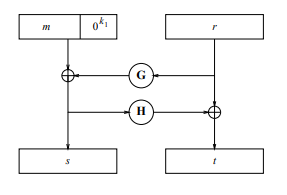
\includegraphics{bibliography.png}
		
		Αναλυτικότερα, έχουμε τα εξής:
		\begin{itemize}
			\item \textbf{{\lt{G}}}: μία {\lt{hash function}} με {\lt{output g bits}} 
			\item \textbf{{\lt{H}}}: μία {\lt{hash function}} με {\lt{output h bits}}
			\item \textbf{{\lt{r}}}: μία συμβολοσειρά μήκους {\lt{g bits}}
		\end{itemize}
	
		Έστω \textbf{{\lt{m}}} το μήνυμα που θέλουμε να κρυπτογραφήσουμε με μήκος {\lt{bits}} μικρότερο από {\lt{g bits}}.
		
		Αρχικά, δημιουργούμε το καινούριο μήνυμα \textbf{{\lt{m'}}}, το οποίο αποτελεί το παλιό μήνυμα {\lt{m}} στο οποίο έχουμε προσθέσει στο τέλος (έχουμε κάνει \textbf{{\lt{append}}}) όσα \textbf{μηδενικά} χρειάζεται για να φτάσουμε το νέο μήνυμα \textbf{να είναι μήκους {\lt{g bits}}}.
		
		Στη συνέχεια δημιουργούμε:	
		\begin{itemize}
			\item To \textbf{{\lt{s}}} το οποίο παράγεται κάνοντας: \textbf{{\lt{m' XOR G(r)}}}.
			\item To \textbf{{\lt{t}}} το οποίο παράγεται κάνοντας: \textbf{{\lt{r XOR H(m' XOR G(r))}}}.
		\end{itemize}
	
		Τέλος, δημιουργούμε το \textbf{{\lt{Χ}}} το οποίο αποτελεί την ένωση του \textbf{{\lt{s || t}}} (δηλαδή {\lt{s append t}}), και μετά κρυπτογραφούμε το {\lt{X}} χρησιμοποιώντας το \textbf{\lt{RSA}} και στέλνουμε το κρυπτογραφημένο μήνυμά μας.
		
		{\lt{ref}}:
		{\lt{\href{ftp://ftp.di.ens.fr/pub/users/pointche/Papers/2002_cryptobytes.pdf}{2002-cryptobytes}}}
		
		
		\item \textbf{Να μελετήσετε βιβλιογραφικα τις στρατηγικές {\lt{first sign then encrypt}} \& {\lt{first encrypt then sign}} και να καταλήξετε σε κάποια συμπεράσματα (πλεονεκτήματα/μειονεκτήματα)}
		
		\begin{itemize}
			\item Κατα την στρατηγική \textbf{\lt{first sign then encrypt}}, η λογική είναι η εξής:
		\end{itemize}
		
		Ο αποστολέας μαζί με το μήνυμά του, βάζει επίσης την ψηφιακή υπογραφή του. Στη συνέχεια, και τα δύο αυτά μαζί τα κρυπτογραφεί και τα στέλνει σε κάποιον παραλήπτη.
		
		\begin{itemize}
			\item Κατα την στρατηγική \textbf{\lt{first encrypt then sign}}, η λογική είναι η εξής:
		\end{itemize}
		
		Ο αποστολέας κρυπτογραφεί το μήνυμά του, στη συνέχεια βάζει την ψηφιακή υπογραφή του μαζί με το κρυπτογραφημένο πια μήνυμα και τα στέλνει σε κάποιον παραλήπτη.
		
		\textbf{Ανάλυση}\\
		Όταν χρησιμοποιούμε την \textbf{\lt{first sign then encrypt}} στρατηγική, είναι προφανές ότι η ψηφιακή μας υπογραφή στέλνεται και αυτή κρυπτογραφημένη στον παραλήπτη. Αυτό σημαίνει πρακτικά ότι μόνο ο παραλήπτης μπορεί να αποκρυπτογραφήσει το μήνυμα και μετά να επιβεβαιώσει την ψηφιακή υπογραφή μου, ενώ αν κάποιος τρίτος πάρει στα χέρια του το {\lt{cipher-text}}, δεν μπορεί να βγάλει κανένα συμπέρασμα ούτε για το μήνυμα ούτε για το ποιανού είναι η υπογραφή.
		
		Όταν χρησιμοποιούμε την \textbf{\lt{first encrypt then sign}} στρατηγική ωστόσο, η ψηφιακή μας υπογραφή στέλνεται μη-κρυπτογραφημένη μαζί με το κρυπτογραφημένο μήνυμα στον παραλήπτη. Αυτό σημαίνει ότι αν κάποιος τρίτος πάρει στα χέρια του το {\lt{cipher-text}} του μηνύματος μαζί με την υπογραφή μου, μπορεί να δει ότι κάτι έχω υπογράψει αλλά δεν μπορεί φυσικά να δει το περιεχόμενο του μηνύματος.
		
		\textbf{Συμπεράσματα}\\
		Καταλήγουμε λοιπόν στο συμπέρασμα ότι δεν υπάρχει σωστή η λάθος στρατηγική ανάμεσα στις δύο, καθώς εξαρτάται από το τι θέλουμε να πετύχουμε. Η κοινή λογική λέει πως από τι στιγμή που στέλνουμε ένα κρυπτογραφημένο κείμενο σε κάποιον, θέλουμε ένας τρίτος που πάρει στα χέρια του το {\lt{cipher text}} να έχει όσο δυνατόν λιγότερη πληροφορία για αυτό, και άρα η στρατηγική \textbf{\lt{first sign then encrypt}} φαντάζει πιο σωστή.
		
		Για παράδειγμα, αν έχω χρησιμοποιήσει την στρατηγική \textbf{\lt{first encrypt then sign}} και κάποιος τρίτος πάρει στα χέρια του το {\lt{cipher text}} με την υπογραφή μου που έστειλα στον παραλήπτη {\lt{Χ}}, μπορεί να αλλάξει την υπογραφή μου, να εισάγει την υπογραφή του, και να στείλει το {\lt{cipher text}} στον παραλήπτη {\lt{Χ}} ως δικό του. Αυτό ελλωχεύει τον κίνδυνο ο {\lt{Χ}} να έρθει σε επαφή με τον τρίτο, καθώς νομίζει ότι αυτός του έστειλε το {\lt{cipher-text}} που αρχικά έστειλα εγώ, και να του αποκαλύψει άθελά του πληροφορίες για το αποκρυπτογραφημένο μήνυμα.
		
		Ο μόνος λόγος για να χρησιμοποιήσουμε την στρατηγική \textbf{\lt{first encrypt then sign}} θα ήταν εάν δεν θα μας πείραζε ή ακόμη καλύτερα αν θα θέλαμε να φαίνεται σε όλους, σε οποιονδήποτε μπορεί να πάρει το {\lt{cipher-text}}, ότι το μήνυμα αυτό το έχω υπογράψει εγώ.
	\end{enumerate}
	
	\addcontentsline{toc}{section}{Θέμα 22}
	\section*{{\color{maroon}Θέμα 22}}
	\section*{\lt{3.1}}
	{\lt{
			Αρχικά θέλουμε να αποδείξουμε ότι οι αριθμοί της μορφής $4n+3$ δεν είναι τέλεια τετράγωνα.
			Αρχικά για $n\leq0$ εύκολα παρατηρούμε ότι ισχύει η παραπάνω πρόταση. Αυτό συμβαίνει καθώς για $n=0$ έχουμε το $3$ το οποίο δεν είναι τέλειο τετράγωνο και για $n < 0$ το $4n+3$ είναι αρνητικός. 
			
			Έστω ότι,
			$$4n+3=a^2, \quad n,a \in \mathbb{N}^* (1)$$
			
			Εφόσον $a\in \mathbb{N}^*$, τότε μπορούμε να πούμε ότι $a=2k+1, \quad k \in \mathbb{N}$.
			
			Αντικαθιστώντας το $a$ στην (1) έχουμε:
			\begin{gather*}
			4n+3 = (2k+1)^2 \implies 4n+3 = 4k^2 + 4k + 1 \\
			\equiv 4k^2 + 4k - 4n = 2 \\
			\equiv 2(k^2 + k - n) = 1 \\
			\equiv k^2 + k - n = \frac{1}{2}
			\end{gather*}
			
			Το οποίο είναι άτοπο καθώς $k,n \in \mathbb{N}^*$ και άρα το $k^2\in \mathbb{N}^* $
			αλλά και όλη η παράσταση $k^2 + k - n \in \mathbb{N}$, εφόσον είναι άθροισμα των φυσικών αριθμών $k^2, k$ και $-n$.
			
			Συνεπώς και η αρχική ισοδύναμη υπόθεση είναι άτοπη, οπότε το $4n+3$ δεν είναι τέλειο τετράγωνο.
			
			Για το δεύτερο ερώτημα παρατηρούμε ότι όλοι αριθμοί
			$$11,111,...,111\cdotp\cdotp\cdotp111,...$$ 
			μπορούν να γραφούν στην μορφής $(4n+3) + 10^q$, συνεπώς αυτό το σύνολο αριθμών δεν θα έχει τέλειο τετράγωνο.
	}}
	
	\addcontentsline{toc}{section}{Θέμα 23}
	\section*{{\color{maroon}Θέμα 23}}
	\section*{\lt{3.4}}
	{\lt{
			Υπάρχουν δύο περιπτώσεις που θα χρειαστεί να εξετάσουμε.
			
			Περίπτωση 1:
			Για περιττό αριθμό διαδοχικών αριθμών, αυτοί οι αριθμοί θα έχουν ως μέσο έναν ακέραιο (μεσσαίος αριθμός), οπότε το άθροισμα γράφεται ως εξής:
			$$sum = average * number\_of\_consecutive\_numbers$$
			$$\implies sum = integer * odd\_number$$
			Αυτό σημαίνει ότι το άθροισμα ($sum$) διαιρείται από έναν περιττό αριθμό. Αυτό όμως δεν μπορεί να είναι το σενάριο για το $2^m$.
			
			Περίπτωση 2:
			Ένας ζυγός αριθμός διαδοχικών αριθμών έχουν ως μέσο το μέσο του αθροίσματος των δύο μεσαίων. Συνεπώς έχουμε:
			$$sum = ((sum\_of\_two\_middle\_numbers) * \frac{1}{2}) * number\_of\_consecutive\_numbers$$
			$$\implies sum = (sum\_of\_two\_middle\_numbers) * \frac{1}{2} * even\_number$$
			$$\implies sum = (sum\_of\_two\_middle\_numbers) * integer$$
			$$\implies sum = ((k) + (k+1)) * integer \quad , k \in \mathbb{Z}$$
			$$\implies sum = (2k+1) * integer$$
			Το $2k+1$ είναι περιττός αριθμός, άρα το άθροισμα ($sum$) έχει ως παράγοντα περιττό, άρα όπως και προηγουμένως απορρίπτεται το σενάριο $2^m$.
	}}
	
	\addcontentsline{toc}{section}{Θέμα 24}
	\section*{{\color{maroon}Θέμα 24}}
		\section*{\lt{3.7}}
	{\lt{
			Έστω ότι $$a = n^5 + 1, b = n^{10} - 1, c = n^5 - 1$$
			
			$$a \cdot c = (n^5 + 1)\cdot (n^5 - 1) = n^{5^2} - 1^2 = n^{10} - 1 = b$$
			
			Γνωρίζουμε όμως (από ορισμό 3.1.1) ότι $a|b$ αν υπάρχει ακέραιος αριθμός $c$ τέτοιος ώστε $b = a \cdot c$ . Επομένως, η αρχική πρόταση αποδείχτηκε.
			
	}}
	
	\addcontentsline{toc}{section}{Θέμα 25}
	\section*{{\color{maroon}Θέμα 25}}
		\section*{\lt{3.19}}
	Κώδικας με σχόλια στο αρχείο:
	{\lt{
			$$No25\_Maths\_3\_19.ipynb$$
	}}
	
	\addcontentsline{toc}{section}{Θέμα 26}
	\section*{{\color{maroon}Θέμα 26}}
		\section*{\lt{3.23}}
	{\lt{
			Από την εκφώνηση έχουμε δύο δεδομένα: 
			$$(1)\quad gcd(n,a) = 1$$ 
			$$(2)\quad n | a\cdot b$$
			Χρησιμοποιώντας το 1ο δεδομένο, από την ταυτότητα Bezout, υπάρχουν ακέραιοι x, y, τέτοιοι ώστε $1 = x\cdot n + y\cdot a$. \\
			Οπότε $b = b\cdot x\cdot n + b\cdot y\cdot a$. \\
			Αλλά:\\
			$n | b\cdot x\cdot n$ (εννοείται) και\\
			$n | y\cdot (a\cdot b)$ (χρησιμοποιώντας το 2ο δεδομένο)\\
			Επομένως, $n | b\cdot x\cdot n + b\cdot y\cdot a$, δηλαδή $n|b$.
			
	}}
	
	\addcontentsline{toc}{section}{Θέμα 27}
	\section*{{\color{maroon}Θέμα 27}}
	\section*{\lt{3.26}}
	{\lt{
			\begin{enumerate}[label=(\roman*)]
				\item Έστω ότι $d_1 = \gcd(c,b)$ και $d_2 = \gcd(ac,b)$
				
				Τότε έχουμε $c \cdot x_1+b \cdot y_1 = d_1$, $a \cdot c \cdot x_2+b \cdot y_2 = d_2$ και $a \cdot x+b \cdot y=1$, από Bezout.
				Αρχικά πολλαπλασιάζουμε την $a \cdot x+b \cdot y=1$ με το $d_1$ και έχουμε:
					\begin{gather*}
					d_1 \cdot (a \cdot x+b \cdot y)=1 \cdot d_1 \\
					\implies a \cdot x(c \cdot x_1+b \cdot y_1)+b \cdot d_1 \cdot y = d_1 \\
					\implies a \cdot c \cdot (x \cdot x_1)+b \cdot (a \cdot x \cdot y_1+d_1 \cdot y) = d_1
					\end{gather*}
				Εφόσον ισχύει ότι $d_2 = \gcd(ac,b)$, τότε διαιρεί κάθε ακέραιο γραμμικό συνδυασμό των $ac$ και $b$ και άρα έχουμε $d_2|d_1 \quad(1)$.
				
				Στην συνέχεια θα πολλαπλασιάσουμε ομοίως το $a \cdot x+b \cdot y=1$ με το $d_2$ και έχουμε:
					\begin{gather*}
					d_2 \cdot (a \cdot x+b \cdot y)=1 \cdot d_2 \\
					\implies a \cdot x(a \cdot c \cdot x_2+b \cdot y_2)+b \cdot d_2 \cdot y = d_2 \\
					\implies c \cdot (a^2 \cdot x \cdot x_2) + b \cdot (a \cdot x \cdot y_2 + d_2 \cdot y) = d_2
					\end{gather*}
				Ομοίως με προηγουμένως ισχύει ότι $d_1 = \gcd(c,b)$, τότε διαιρεί κάθε ακέραιο γραμμικό συνδυασμό των $ac$ και $b$ και άρα έχουμε $d_1|d_2 \quad(2)$.
				Από (1) και (2) έχουμε ότι $d_1 = d_2$, μη αρνητικά.
				
				Αφού 
				$$(1) \implies |d_1| \leqslant |d_2|$$
				$$(2) \implies |d_2| \leqslant |d_1|$$
				\item Έστω $d$ κοινός διαρέτης των $a+b$ και $a-b$, τότε ο $d$ διαιρεί και το άθροισμα και την διαφορά τους.
				$$d|(a+b)$$
				$$d|(a-b)$$
				$$d|(a+b)+(a+b) = 2 \cdot a$$
				$$d|(a+b)-(a-b) = 2 \cdot b$$
				
				Τότε έχουμε ότι:
				$$d|\gcd(2a,2b)=2\gcd(a,b)$$
				Όμως από αρχικά δεδομένα έχουμε ότι $\gcd(a,b)=1$ άρα τότε ισχύει:
				$$d|2$$
				Συνεπώς το $d \in \{1,2\}$
				
				Εαν a,b περιττοί τότε έχουμε το εξής:
				$$a = 2k_1+1 \quad k_1 \in \mathbb{Z}$$
				$$b = 2k_2+1 \quad k_2 \in \mathbb{Z}$$	
				Άρα θα ισχύει και το εξής:
				$$a+b = 2k_1+1 + 2k_2+1 = 2k_1 + 2k_2 + 2 = 2\cdot (k_1+k_2+1) \quad (even)$$
				$$a-b = 2k_1+1 - 2k_2+1 = 2k_1 - 2k_2 = 2\cdot (k_1 - k_2) \quad (even)$$
				Εφόσον και τα δύο είναι ζυγοί αριθμοί τότε οι διαιρέτες τους θα είναι ζυγοί.
				Όπως αποδείξαμε προηγούμενος όμως, αν $d$ διαιρέτης, τότε $d \in \{1,2\}$
				Συμπερασματικά έχουμε ότι $d=2$.
				
				\item Έστω $d=\gcd(a,b)$ τότε $d=a\cdot x + b\cdot y, \quad x,y \in \mathbb{Z}$
				Αν $i=\gcd(2^a-1, 2^b-1)$ τότε
				$$2^a \equiv 1 \mod{i}$$
				$$2^b \equiv 1 \mod{i}$$
				Συνεπώς έχουμε
				$$2^d = 2^{a\cdot x + b\cdot y} = (2^a)^x \cdot (2^b)^y \equiv 1 \mod{i}$$
				Οπότε $p|2^d-1$.
				Από την άλλη μεριά αν $d|a$, τότε $2^d-1|2^q-1$, οπότε το $2^d-1$ αποτελεί κοινό παράγοντα.
				Έτσι αποδείξαμε ότι 
				$$\gcd(2^a-1,2^b-1)=2^{\gcd(a,b)}-1$$
				Όμως από αρχικά δεδομένα $d=1$, άρα και η προηγούμενη σχέση γράφεται:
				$$\gcd(2^a-1,2^b-1)=1$$
				\item Παρατηρούμε ότι αν αντικαταστήσουμε τα $M_p, M_q$ έχουμε την παραπάνω σχέση.
			\end{enumerate}
	}}
	
	\addcontentsline{toc}{section}{Θέμα 28}
	\section*{{\color{maroon}Θέμα 28}}
		\section*{\lt{3.40}}
	Κώδικας με σχόλια στο αρχείο:
	{\lt{
			$$No28\_Maths\_3\_40.ipynb$$
	}}
	
	\addcontentsline{toc}{section}{Θέμα 29}
	\section*{{\color{maroon}Θέμα 29}}
		\section*{\lt{3.42}}
	Κώδικας με σχόλια στο αρχείο:
	{\lt{
			$$No29\_Maths\_3\_42.ipynb$$
	}}
	
	\addcontentsline{toc}{section}{Θέμα 30}
	\section*{{\color{maroon}Θέμα 30}}
	\section*{\lt{3.70}}
	{\lt{
			Υπόθεση:\\
			$
			N>2 \\
			N = p_1p_2\ldots p_k \\
			p_j-1|N-1 \forall j
			$\\
			Απόδειξη:\\
			Έστω $\gcd(a,N)=1$. \\
			Από το θεώρημα του Fermat, $\forall j$, έχουμε $a^{p_j} \equiv 1 \mod{p_j}$.\\
			Εφόσον $p_j-1|N-1$,και άρα $a^{N-1}\equiv 1 \mod{p_j}$. \\
			Δηλαδή το $a^{N-1}-1$ είναι πολλαπλάσιο κάθε $p_j$. \\
			Συνεπώς $a^{N-1}\equiv 1 \mod{Ν}$.
	}}
	
	\addcontentsline{toc}{section}{Θέμα 31}
	\section*{{\color{maroon}Θέμα 31}}
	\section*{\lt{3.74}}
	{\lt{
			Παρατηρούμε ότι $561(=3\cdot 11 \cdot 17)$ είναι αριθμός Carmichael. Θα βρούμε όλους του αριθμούς Carmichael μέχρι $Ν(=3000)$.
			
			Πρόταση 1:
			Έστω $n=p \cdot u$ όπου $p$ είναι πρώτος. Τότε αν και μόνο αν $p-1|u-1$ θα ισχύει και $p-1|n-1$.
			$$(n-1)-(u-1) = n-u = p\cdot u-u=(p-1)\cdot u$$
			
			Πρόταση 2:
			Έστω ένας αριθμός Carmichael έχει τουλάχιστον τρεις πρώτους παράγοντες. Για την απόδειξη αυτής της πρότασης εφαρμόζουμε την εξής λογική:
			
			Έστω ότι ο $n$ έχει δύο πρώτους παράγοντες $n=p\cdot q$ όπου $p,q$ πρώτοι και $p>q$. Τότε $p-1 > q-1$, άρα το $p-1$ δεν διαιρεί το $q-1$. Από την πρόταση (1) το $p-1$ δεν διαιρεί το $n-1$. Συνεπώς το $n$ δεν είναι αριθμός Carmichael.
			
			Πρόταση 3:
			Ας υποθέσουμε ότι ο $n$ είναι Carmicael και ότι το $p$ και το $q$ είναι πρώτοι παράγοντες του n. Τότε $q\not\equiv 1 \mod p$.
			
			Έστω ότι το $q\equiv 1 \mod p$, έτσι ισχύει ότι $p|q-1$. Τότε $q-1|n-1$ καθώς θα ισχύει και ότι $p|n-1$. Όμως αυτό είναι άτοπο καθώς ισχύει ότι $p|n$.
			
			Εύρεση αριθμών Carmichael:
			Έστω αριθμός $n$ με τρεις πρώτους παράγοντες $n=p\cdot q\cdot r$ , με $p<q<r$. Από τα προηγούμενα καταλαβαίνουμε ότι χρειαζόμαστε τριπλέτες $(p,q,r)$ για τις οποίες θα ισχύουν τα εξής:
			
			\begin{gather*}
			(i) \quad p-1|q\cdot r-1 \quad (or \quad q\cdot r \equiv 1 \mod (p-1)) \\ 
			(ii) \quad q-1|p\cdot r-1 \\ 
			(iii) \quad r-1|p\cdot q-1 
			\end{gather*}
			
			Δοθεί ένα ζευγάρι πρώτον αριθμών $(p,q)$ με $p<q$, η ακόλουθη διαδικασία θα εντωπίσει όλους τους πρώτους $r>q$ τέτοιοι ώστε το $p\cdot q\cdot r$ να είναι αριθμός Carmichael.
			
			Έστω οι ζυγοί διαρέτες (αν υπάρχουν) $d$ του $p\cdot q -1$ με $p<d<p\cdot q -1$ και ελέγχουμε αν $d+1 (=r)$ είναι πρώτος, εξαιρούμε το $d=p\cdot q-1$ καθώς θα μας έδινε $r=p\cdot q$. Τότε έχουμε εξασφαλίσει το (iii) και ελέγχουμε λοιπόν αν ισχύουν τα (ii) και (ii).
			
			Το κάνουμε για όλα τα ζευγάρια πρώτων $(p,q)$, όπου $p\cdot q\cdot r < 3000$, για πρώτους $r>q$. Όμως λόγω του (3) αφήνουμε εκτός τους συνδυασμούς για τους οποίους ισχύει: $q \equiv 1 \mod p$ (π.χ $(3,7)$).
			
			Καταγράφουμε μόνο τις τιμές του $d$ όπου το $r$ είναι πρώτος.
			Όπως παρατηρούμε και στον πίνακα από κάτω δεν υπάρχει μικρότερος  Carmichael με τρείς παράγοντες από τον 561.
			\begin{center}
				\begin{tabular}{||c c c c c c c||} 
					\hline
					$(p,q)$ & $p\cdot q-1$ & $d$ & $r$  & (i) & (ii)  & Carmichael \\ [0.5ex] 
					\hline\hline
					$(3,5)$ & $14$ & $-$ & $-$ &  &  &  \\ 
					\hline
					$(3,11)$ & $32$ & $16$ & $17$ & yes & yes & $3\cdot 11 \cdot 17 = 561$ \\
					\hline
					$(3,17)$ & $50$ & $-$ & $-$ &  &  &  \\
					\hline
					$(3,23)$ & $68$ & $-$ & $-$ &  &  &  \\
					\hline
					$(5,7)$ & $34$ & $-$ & $-$ &  &  &  \\ [1ex] 
					\hline
					$(5,13)$ & $64$ & $16$ & $17$ & yes & yes & $5\cdot 13 \cdot 17 = 1105$ \\ [1ex] 
					\hline
					$(5,17)$ & $84$ & $28$ & $29$ & yes & yes & $5\cdot 17 \cdot 29 = 2465$ \\ [1ex] 
					\hline
					$ $ & $ $ & $42$ & $43$ & no &  &  \\ [1ex] 
					\hline
					$(5,19)$ & $94$ & $-$ & $-$ &  &  &  \\ [1ex] 
					\hline
					$(7,11)$ & $76$ & $-$ & $-$ &  &  &  \\ [1ex] 
					\hline
					$(7,13)$ & $90$ & $18$ & $19$ & yes & yes & $7\cdot 13 \cdot 19 = 1729$ \\ [1ex] 
					\hline
					$ $ & $ $ & $30$ & $31$ & yes & yes & $7\cdot 13 \cdot 31 = 2821$ \\ [1ex] 
					\hline
					$(7,17)$ & $118$ & $-$ & $-$ &  &  &  \\ [1ex] 
					\hline
					$(11,13)$ & $142$ & $-$ & $-$ &  &  &  \\ [1ex] 
					\hline
					
				\end{tabular}
			\end{center}
			
			Το δεύτερο ερώτημα επιλύθηκε με βοήθεια κώδικα.

			Κώδικας με σχόλια στο αρχείο:
			{\lt{
					$$No31\_Smaller\_Carmichael\_4\_Factors.ipynb$$
			}}
	}}
	
	\bibliographystyle{plain}
	\bibliography{bib.bib}
	
\end{document} 
